\documentclass[12pt,a4paper]{article}

\usepackage[utf8]{inputenc}
\usepackage[T1]{fontenc}
\usepackage[french]{babel}
\usepackage{amsmath,amssymb,amsthm}
\usepackage{cmbright} % whole document sans-serif, matching sans math
\usepackage{exscale}
\usepackage[hidelinks]{hyperref}
\usepackage{cleveref}
\usepackage{graphicx}
\usepackage{xcolor}
\definecolor{accent}{HTML}{244470} % not exactly navy blue, but better imo
\usepackage{geometry}
\geometry{hmargin=2cm,vmargin=2cm}

\usepackage{titlesec}
% Style the sections with the navy color
\titleformat{\section}
  {\color{accent}\Large\bfseries}
  {\thesection.}
  {0.8em}
  {}
\titleformat{\subsection}
  {\color{accent}\large\bfseries}
  {\thesubsection}
  {0.7em}
  {}

\usepackage[many]{tcolorbox}
% Create a box that is white, but has a 3pt navy line on the left
\tcbset{
  navybar/.style={
    enhanced,
    colback=white,
    colframe=accent,
    boxrule=0pt,
    leftrule=3pt,
    arc=0pt,
    outer arc=0pt,
    left=8pt, right=8pt, top=6pt, bottom=6pt
  }
}

% Theorems and definitions
\theoremstyle{plain}
\newtheorem{theorem}{Théorème}[section]

\theoremstyle{definition}
\newtheorem{definition}[theorem]{Définition}
\newtheorem{example}[theorem]{Exemple}

\newtheorem{exercise}{Exercice}

\theoremstyle{remark}
\newtheorem*{remark}{Remarque}
\newtheorem*{recall}{Rappel}

\begin{document}

\noindent
\begin{minipage}[c]{0.62\textwidth}
  {\color{accent}\LARGE\bfseries Activités Numériques\par}
  \vspace{0.1cm}
  {\large 1\textsuperscript{ère} année secondaire\par}
  \vspace{0.7cm}
  {\bfseries \href{https://www.linkedin.com/in/kefrov/}{Fares Manai}\par}
  \vspace{2pt}
  {\small\href{mailto:kefrov630@gmail.com}{kefrov630@gmail.com}\par}
\end{minipage}
\hfill
\begin{minipage}[c]{0.26\textwidth}
  \centering
  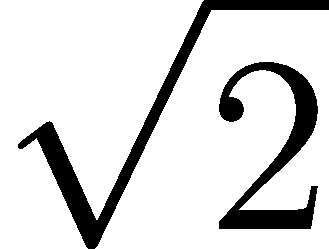
\includegraphics[width=\linewidth]{sqrt2.pdf}
\end{minipage}
\par\vspace{0.4cm}
\noindent{\color{accent}\rule{\linewidth}{0.9pt}}
\par\vspace{0.5cm}


\renewcommand{\contentsname}{Sommaire}
\tableofcontents

\newpage
\section*{Introduction}
\addcontentsline{toc}{section}{Introduction}

\newpage
% \texorpdfstring{}{} is cool for pdf bookmarks
\section{Arithmétique dans \texorpdfstring{\(\mathbb{N}\)}{N}}

\subsection{Les Ensembles}

Les mathématiques étudient la logique, les régularités et les relations
entre des objets mathématiques. Les ensembles permettent de regrouper ces
objets. À notre niveau, on peut voir un ensemble comme une collection
d'éléments, à condition que ces éléments soient bien définis.

\begin{example}
  Soit $E$ l'ensemble des entiers pairs de 1 à 10 :
  \[
    E = \{2, 4, 6, 8, 10\}.
  \]
  La notation $x \in E$ signifie que $x$ est un élément de $E$.
  Ici, $x$ peut être n'importe lequel des cinq éléments de $E$.
  De même, $X \subseteq E$ signifie que $X$ est une partie de $E$,
  c'est-à-dire que chaque élément de $X$ appartient aussi à $E$.
  Par exemple, $\{4, 8\} \subseteq E$.
  \label{eg1.1}
\end{example}

Voici deux propriétés importantes des ensembles :

\begin{enumerate}
    \renewcommand{\labelenumi}{(\roman{enumi})}
    \item L'ordre n'a pas d'importance, e.g., $\{1,2\}=\{2,1\}$.
    \item Les répétitions ne changent pas l'ensemble, e.g., 
    $\{1,2,2\}=\{1,2\}$.
\end{enumerate}

L'intersection de deux ensembles, notée $\cap$, est l'ensemble des
éléments qui appartiennent aux deux ensembles. La réunion de deux
ensembles, notée $\cup$, est l'ensemble des éléments qui appartiennent
à au moins un des deux ensembles. Parfois, on veut garder les éléments
d'un ensemble qui n'appartiennent pas à un autre. Pour cela, on utilise
le symbole $\setminus$.

\begin{example}
  Soit $A = \{1, 2, 3, 4\}$ et $B = \{2, 4, 5, 6\}$.
  On obtient :
  \[
    \begin{aligned}
        A \cap B &= \{2, 4\} \\
        A \cup B &= \{1, 2, 3, 4, 5, 6\} \\
        B \setminus A &= \{5, 6\} \\
        A \setminus B &= \{1, 3\}.
    \end{aligned}
  \]
\end{example}

On note $\mathbb{N}$ l'ensemble des entiers naturels :
\[
  \mathbb{N} = \{0, 1, 2, 3, \dots\}.
\]
Les points de suspension $\dots$ indiquent que la suite continue de la
même façon : chaque nombre est égal au précédent plus un.

La notation de l'exemple suivant sert à décrire des ensembles dont les
éléments vérifient des conditions précises.

\begin{example}
  Soit $E$ le même ensemble que dans \cref{eg1.1}. On peut aussi écrire
  \[
    E = \{x \in \mathbb{N} \mid x \text{ est pair et } 1 \le x \le 10\}.
  \]
  La partie avant le symbole $\mid$ donne la variable et l'ensemble
  auquel elle appartient. La partie après $\mid$ donne les conditions
  que la variable doit vérifier. Considérons maintenant l'ensemble
  suivant :
  \[
    F = \{x \in E \mid x \text{ est impair}\}.
  \]
  Cet ensemble n'a aucun élément, car aucun entier ne peut être à la
  fois pair et impair. Donc $F = \varnothing$, où $\varnothing$ désigne
  l'ensemble vide. On peut aussi écrire l'ensemble vide $\{\}$.
\end{example}

\begin{remark}
  Notons que $0 \in \mathbb{N}$. Pour parler des entiers naturels
  strictement positifs, on utilise la notation $\mathbb{N}^*$ :
  \[
    \mathbb{N}^* = \mathbb{N} \setminus \{0\}
    = \{1, 2, 3, \dots\}.
  \]
\end{remark}

\newpage
\section*{Conclusion}
\addcontentsline{toc}{section}{Conclusion}

\end{document}
